\documentclass[12pt,a4paper]{article}
\usepackage[utf8]{inputenc}
\usepackage[T5]{fontenc}
\usepackage[vietnamese]{babel}
\usepackage{graphicx,float,geometry,array,booktabs,enumitem,amsmath,amssymb,hyperref,tocloft,titlesec}
\newcommand{\sectionbreak}{\clearpage}
\geometry{top=2cm,bottom=2cm,left=2.5cm,right=2cm}
\hypersetup{colorlinks=true,linkcolor=black,citecolor=black,urlcolor=blue}
\graphicspath{{hinh/}}
\setlist{nosep,leftmargin=1.5em}
\setlength{\cftbeforesecskip}{2pt}
\setlength{\cftbeforesubsecskip}{1pt}
\setlength{\parindent}{1.2cm}
\setlength{\parskip}{3pt}
\tolerance=2000
\emergencystretch=2em

\begin{document}
\begin{titlepage}
\begin{center}
{\Large ĐẠI HỌC BÁCH KHOA HÀ NỘI}\\[0.5cm]
{\textbf{\large TRƯỜNG CÔNG NGHỆ THÔNG TIN VÀ TRUYỀN THÔNG}}\\[1.8cm]

\includegraphics[width=3.2cm]{hinh0.png}\\[1cm]
{\Huge \textbf{BÁO CÁO PROJECT II}}\\[0.8cm]
{\LARGE \textbf{Đề tài:}}\\[0.3cm]
\parbox{0.92\textwidth}{\centering\Large\textbf{NGHIÊN CỨU SO SÁNH CÁC KIẾN TRÚC PYTORCH CHO BÀI TOÁN PHÂN LOẠI CẢM XÚC ĐA NHÃN TRÊN GOEMOTIONS}}
\vfill
\begin{tabular}{rl}
\textbf{Người thực hiện:} & Nguyễn Nhật Trung \\[0.3cm]
\textbf{Giảng viên hướng dẫn:} & TS. Nguyễn Duy Hiệp
\end{tabular}
\vfill
{\large Hà Nội, tháng 08 năm 2026}
\end{center}
\end{titlepage}

\tableofcontents
\clearpage

\section{Giới thiệu}
\subsection{Bài toán và động lực}

Nhận diện cảm xúc trong văn bản được sử dụng trong phân tích phản hồi, theo dõi cộng đồng và xây dựng trợ lý hội thoại. Khác với bài toán phân loại cảm xúc (sentiment analysis) thường chỉ chia văn bản thành tích cực, tiêu cực và trung tính, nhân diện cảm xúc (emotion classification) cần phân biệt các trạng thái chi tiết như joy, sadness, anger, surprise, fear,... Một câu cũng có thể đồng thời thể hiện nhiều cảm xúc. Vì vậy, đầu ra của hệ thống là một tập nhãn không phải duy nhất một lớp.

GoEmotions gồm 27 loại cảm xúc và nhãn \textit{neutral}, được gán cho các bình luận tiếng Anh trên Reddit \cite{demszky2020}. Bộ nhãn chi tiết làm bài toán khó vì phân bố nhãn mất cân bằng, nhiều nhãn gần nghĩa và câu ngắn thường thiếu ngữ cảnh. Project xây dựng bốn hệ thống từ biểu diễn thống kê đến neural network huấn luyện từ đầu: TF-IDF kết hợp Logistic Regression, Mean Pooling MLP, BiLSTM kết hợp attention và Transformer Encoder. BERT-base-cased pretrained được fine-tune làm mốc tham chiếu bên ngoài của bài báo gốc.

\subsection{Mục tiêu của báo cáo}

Báo cáo tập trung trả lời các câu hỏi thực hành:
\begin{enumerate}
\item Dữ liệu được kiểm tra, làm sạch và chuyển thành đầu vào cho mô hình như thế nào?
\item Khi tăng khả năng biểu diễn từ TF-IDF đến MLP, BiLSTM và Transformer, chất lượng thay đổi ra sao?
\item Các mô hình huấn luyện từ đầu đứng ở đâu so với BERT pretrained của bài báo gốc?
\item Vì sao threshold 0.5 chưa phù hợp cho mọi nhãn và tuning threshold cải thiện kết quả như thế nào?
\item Những nhãn và loại mẫu nào vẫn gây khó cho hệ thống?
\end{enumerate}

Kết quả được chọn bằng validation macro-F1. Test chỉ dùng sau khi cấu hình và threshold đã đóng băng. BERT không được coi là mô hình ngang bằng hoàn toàn với nhóm train-from-scratch vì đã học kiến thức ngôn ngữ từ lượng văn bản lớn trước khi fine-tune trên GoEmotions.

\section{Dữ liệu và quy trình xử lý}
\subsection{Nguồn dữ liệu và cấu trúc nhãn}

Project sử dụng configuration \texttt{simplified} của \texttt{google-research-datasets/go\_emotions} với official train/validation/test splits. Mỗi dòng có nội dung \texttt{text}, danh sách mã nhãn \texttt{labels} và mã mẫu \texttt{id}. Thứ tự 28 nhãn được lấy từ dataset feature và đóng băng cho toàn bộ pipeline. Cột thứ $j$ trong target, logit, probability và threshold luôn cùng chỉ một nhãn.

Một target là vector multi-hot độ dài 28. Nếu câu có cả \textit{caring} và \textit{optimism}, hai vị trí tương ứng bằng 1 và các vị trí còn lại bằng 0. Đây là multi-label classification: mô hình phải giải quyết 28 quyết định nhị phân có liên quan trên mỗi câu.

\subsection{Kiểm tra và tạo clean splits}

Trước khi train, project kiểm tra schema, kiểu dữ liệu, nhãn rỗng hoặc ngoài phạm vi và văn bản trùng lặp. Official splits được giữ nguyên vai trò, nhưng mẫu validation hoặc test có nội dung xuất hiện ở split trước đó bị loại khỏi evaluation view. Mục tiêu là tránh chấm mô hình trên một câu đã nhìn thấy khi train.

Sau xử lý, số mẫu lần lượt là 43.410 train, 5.383 validation và 5.385 test. Vocabulary, IDF, trọng số lớp và mọi tham số học từ dữ liệu chỉ sử dụng train. Validation dùng để chọn mô hình và threshold; test dùng để báo cáo kết quả cuối.

\begin{table}[H]
\centering
\small
\begin{tabular}{lrrr}
\toprule
\textbf{Split} & \textbf{Official} & \textbf{Loại do trùng xuyên split} & \textbf{Clean} \\
\midrule
Train & 43,410 & 0 & 43,410 \\
Validation & 5,426 & 43 & 5,383 \\
Test & 5,427 & 42 & 5,385 \\
\bottomrule
\end{tabular}
\caption{Số mẫu trước và sau khi tạo text-disjoint evaluation views}
\label{tab:clean-splits}
\end{table}


Bảng~\ref{tab:clean-splits} chỉ đếm các mẫu bị loại vì nội dung trùng với một split đứng trước trong evaluation pipeline. Project không xóa các bản ghi trùng nằm hoàn toàn trong cùng một split: mục tiêu của bước này là bảo đảm train, validation và test không chia sẻ nguyên văn, không phải khử trùng lặp toàn bộ dataset.

\begin{figure}[H]
\centering
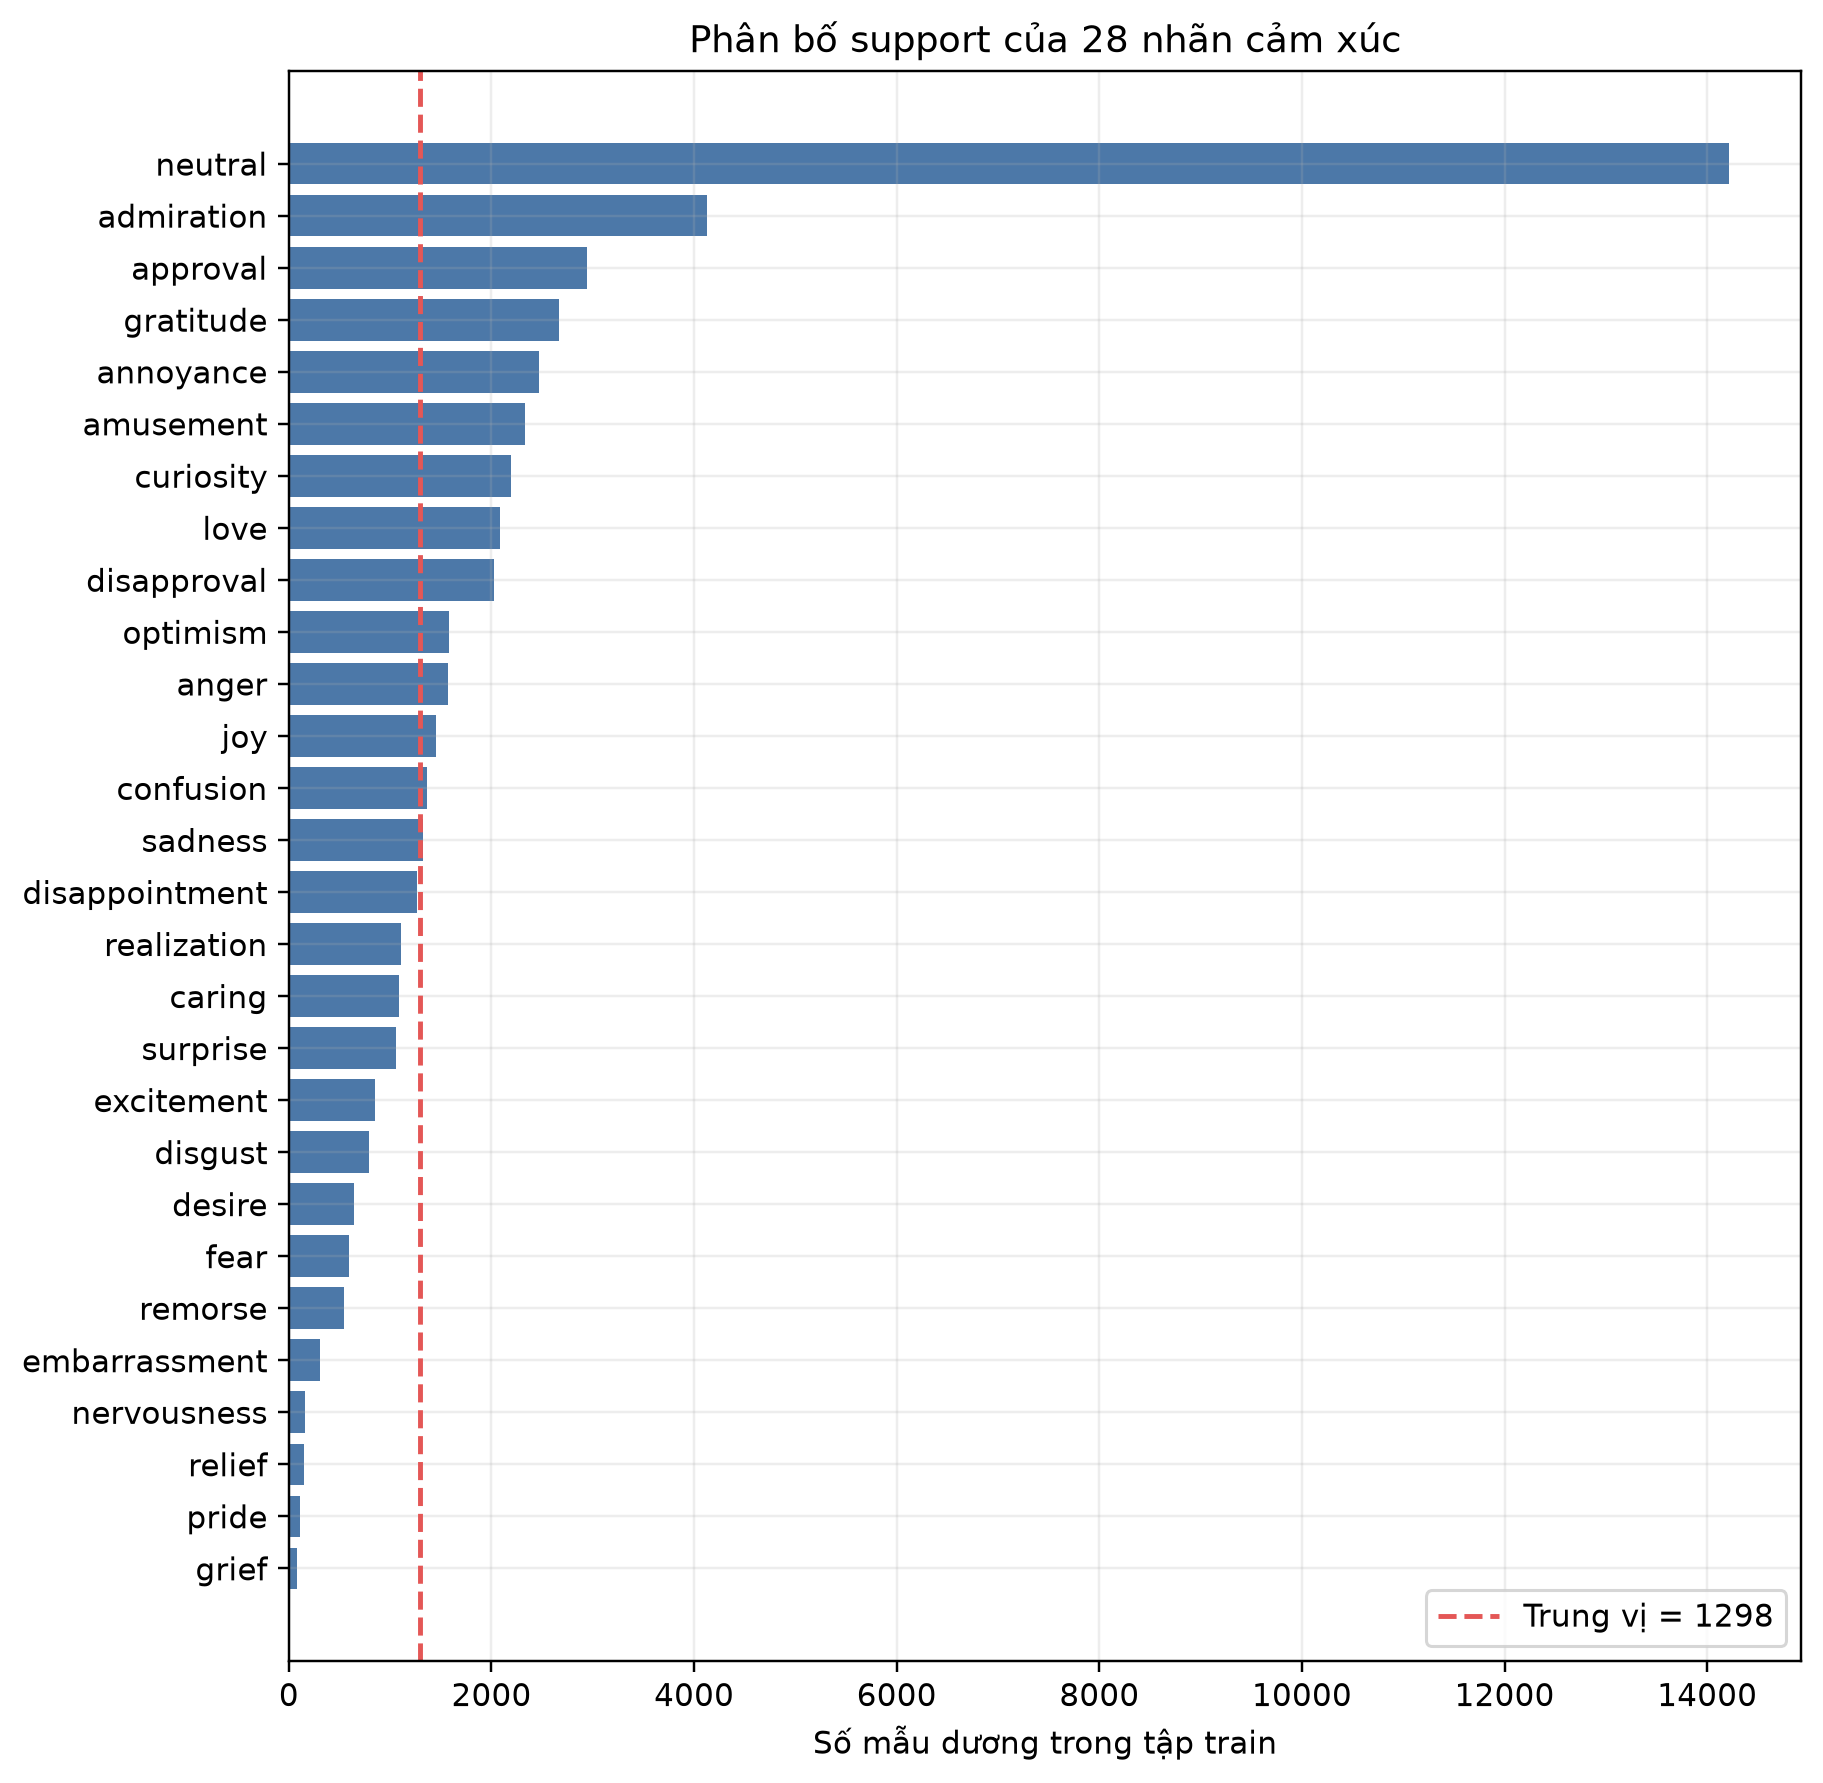
\includegraphics[width=0.86\textwidth]{label_distribution.png}
\caption{Phân bố support của 28 nhãn trong tập train}
\label{fig:label-distribution}
\end{figure}

Hình~\ref{fig:label-distribution} cho thấy \textit{neutral} và một số cảm xúc phổ biến có nhiều mẫu hơn hẳn \textit{grief}, \textit{pride}, \textit{relief} và \textit{nervousness}. Mất cân bằng giải thích vì sao model dễ học nhãn phổ biến nhưng có thể không dự đoán lần nào cho nhãn hiếm khi dùng threshold 0.5.

\subsection{Tokenize và build vocabulary cho mô hình train-from-scratch}

Ba mô hình mạng nơ-ron được xây dựng sử dụng chung một bộ tokenizer dựa trên biểu thức chính quy (Regular Expression). Văn bản được chuyển về chữ thường, sau đó tách thành từ, từ có dấu nháy và dấu câu. Ví dụ, \texttt{I'm happy!} được tách thành \texttt{i'm}, \texttt{happy} và \texttt{!}. Giữ dấu câu hữu ích vì dấu chấm than hoặc dấu hỏi có thể mang tín hiệu cảm xúc.

Vocabulary chỉ được build từ train. Project đếm tần suất token, giữ token xuất hiện ít nhất hai lần, sắp xếp theo tần suất rồi gán integer ID. \texttt{<PAD>} bổ sung vị trí trống để các câu trong batch có chiều dài bằng nhau; \texttt{<UNK>} thay token không xuất hiện trong vocabulary train.

Mỗi câu được biến thành dãy \texttt{input\_ids}. Câu dài hơn giới hạn bị cắt, câu ngắn hơn được padding (thêm \texttt{<PAD>}). \texttt{attention\_mask} bằng 1 ở token thật và bằng 0 ở padding. Mask bảo đảm padding không tham gia mean pooling, attention pooling hoặc self-attention. Validation và test chỉ dùng vocabulary train nên không gây rò rỉ thông tin.

\subsection{Biểu diễn TF-IDF}

TF-IDF dùng tokenizer và vocabulary riêng của \texttt{TfidfVectorizer}. Vectorizer chỉ \texttt{fit} trên train để xác định unigram và inverse document frequency. Token xuất hiện trong ít văn bản có IDF lớn hơn; token xuất hiện gần như mọi nơi có IDF nhỏ hơn. Khi \texttt{transform} validation hoặc test, chỉ feature đã có trong vocabulary train được dùng.

Project thử unigram và unigram--bigram với \texttt{min\_df=2}; unigram được chọn bằng validation macro-F1. Mỗi câu trở thành vector sparse 13.077 chiều. Biểu diễn này nắm bắt tốt từ khóa cảm xúc nhưng không thể hiện trực tiếp thứ tự dài hạn hoặc nghĩa của từ trong ngữ cảnh.

\subsection{WordPiece cho BERT pretrained}

BERT dùng tokenizer \texttt{bert-base-cased}, giữ chữ hoa/chữ thường và tách từ thành WordPiece. Token hiếm có thể được chia thành các mảnh nhỏ đã tồn tại trong vocabulary pretrained. \texttt{[CLS]} được thêm đầu chuỗi, \texttt{[SEP]} đánh dấu cuối chuỗi và \texttt{[PAD]} bổ sung chiều dài. Chuỗi được cắt hoặc padding về tối đa 50 token, đúng cấu hình baseline GoEmotions gốc.

Khác với vocabulary train-from-scratch, WordPiece vocabulary và embedding của BERT đã được học trước. Khi fine-tune, toàn bộ BERT cùng classification head 28 đầu ra được cập nhật. Vì vậy BERT có lợi thế về kiến thức ngôn ngữ và đóng vai trò reference baseline.

\section{Các hệ thống phân loại}
\subsection{Luồng dự đoán chung}

Các neural model nhận \texttt{input\_ids} và \texttt{attention\_mask}, tạo biểu diễn câu rồi sinh 28 logits:
\begin{equation}
\texttt{input\_ids},\ \texttt{attention\_mask}\rightarrow
\texttt{representations}\rightarrow\texttt{logits}\in\mathbb{R}^{B\times28}.
\end{equation}
Targets có shape $[B,28]$ và kiểu \texttt{float32}. \texttt{BCEWithLogitsLoss} nhận logits trực tiếp. Khi đánh giá, sigmoid chuyển logits thành probabilities; threshold quyết định từng nhãn là 0 hay 1.

Với batch gồm $B$ mẫu và $C=28$ nhãn, loss trung bình được viết là
\begin{equation}
\mathcal{L}=-\frac{1}{BC}\sum_{i=1}^{B}\sum_{j=1}^{C}
\left[y_{ij}\log\sigma(z_{ij})+(1-y_{ij})\log\left(1-\sigma(z_{ij})\right)\right].
\end{equation}
Trong đó $z_{ij}$ là logit và $y_{ij}\in\{0,1\}$ là target của nhãn $j$. Khác với \texttt{CrossEntropyLoss} cho multi-class, BCE xem mỗi nhãn như một binary target nên nhiều nhãn có thể đồng thời nhận giá trị 1. Trong triển khai, \texttt{BCEWithLogitsLoss} kết hợp sigmoid và BCE trong một phép tính ổn định số học hơn so với tự sigmoid rồi lấy logarithm.

\subsection{TF-IDF và Logistic Regression}

Mỗi nhãn cảm xúc được huấn luyện bằng một mô hình Logistic Regression độc lập theo chiến lược One-vs-Rest. Đầu vào của mô hình là vector đặc trưng TF-IDF dạng thưa (sparse vector), trong khi đầu ra là xác suất dự đoán cho từng nhãn cảm xúc. Cách tiếp cận này có ưu điểm là đơn giản, dễ triển khai và dễ giải thích, đồng thời hoạt động tốt với những cảm xúc được thể hiện qua các từ khóa hoặc dấu hiệu ngôn ngữ rõ ràng. Tuy nhiên, do các bộ phân loại được huấn luyện độc lập, mô hình không thể hiện được mối quan hệ giữa các nhãn và còn hạn chế trong việc nắm bắt ngữ cảnh. Vì vậy, mô hình được kỳ vọng đạt precision tốt đối với các trường hợp có lexical cues mạnh, nhưng recall có thể thấp hơn ở những nhãn hiếm hoặc các cảm xúc được diễn đạt một cách gián tiếp.

\subsection{Mean Pooling MLP}

Mỗi token ID được ánh xạ sang một vector embedding và các embedding này được học trực tiếp trong quá trình huấn luyện. Attention mask được sử dụng để loại bỏ ảnh hưởng của các token padding, sau đó masked mean pooling tính trung bình các embedding hợp lệ để tạo ra biểu diễn tổng thể cho câu. Vector biểu diễn này tiếp tục được đưa qua một MLP và lớp tuyến tính (linear layer) để sinh ra 28 logits tương ứng với 28 nhãn cảm xúc.

Do sử dụng mean pooling, mô hình không khai thác thông tin về thứ tự và vị trí của các token. Vì vậy, hai câu chứa các token giống nhau nhưng được sắp xếp theo thứ tự khác nhau có thể tạo ra những biểu diễn khá tương đồng. Mô hình MLP này được sử dụng như một neural baseline đơn giản, nhằm đánh giá mức độ cải thiện khi chuyển từ các đặc trưng sparse như TF-IDF sang biểu diễn dense được học trực tiếp từ dữ liệu.

\subsection{BiLSTM kết hợp attention}

BiLSTM xử lý chuỗi theo cả hai chiều, nhờ đó hidden state tại mỗi vị trí có thể tổng hợp thông tin từ cả phần trước và phần sau của câu \cite{hochreiter1997}. Sau đó, attention pooling học mức độ quan trọng của từng token và kết hợp các hidden state thành một vector biểu diễn chung cho toàn câu \cite{bahdanau2015}. So với mean pooling, BiLSTM có khả năng nắm bắt thứ tự từ, trong khi cơ chế attention giúp mô hình tập trung nhiều hơn vào những từ hoặc cụm từ chứa tín hiệu cảm xúc quan trọng. Điều này đặc biệt hữu ích với các câu có cấu trúc phủ định hoặc chứa nhiều tín hiệu cảm xúc khác nhau. Tuy nhiên, embedding đầu vào vẫn được học trực tiếp từ tập dữ liệu GoEmotions, do đó khả năng biểu diễn ngôn ngữ của mô hình vẫn phụ thuộc vào quy mô và đặc điểm của tập dữ liệu này.


\subsection{Transformer Encoder huấn luyện từ đầu}

Mô hình Transformer được xây dựng với token embedding, positional embedding, hai encoder layer, bốn attention head, hidden size 128 và kích thước feed-forward 256. Cơ chế self-attention cho phép mỗi token tương tác và trao đổi thông tin với tất cả các token còn lại trong câu, từ đó giúp mô hình học được các mối quan hệ ngữ cảnh tốt hơn \cite{vaswani2017}. Sau các encoder layer, masked mean pooling được sử dụng để tổng hợp các biểu diễn token thành một vector biểu diễn chung cho toàn câu trước khi đưa vào classification head. So với các baseline đơn giản hơn, kiến trúc này có khả năng mô hình hóa quan hệ giữa các từ trong câu hiệu quả hơn. Tuy nhiên, toàn bộ vocabulary và các trọng số của mô hình đều được học trực tiếp từ tập GoEmotions, nên khả năng biểu diễn vẫn bị giới hạn bởi quy mô và đặc điểm của tập dữ liệu này.

\subsection{BERT-base-cased pretrained}

BERT-base-cased gồm 12 Transformer layer, hidden size 768 và 12 attention head \cite{devlin2019}. Trong project, mô hình được khởi tạo từ checkpoint đã pretrain sẵn, sau đó sử dụng biểu diễn của token \texttt{[CLS]} làm đầu vào cho classification head gồm 28 nhãn cảm xúc. Toàn bộ mô hình được fine-tune trên tập GoEmotions bằng hàm loss Binary Cross-Entropy (BCE). Cấu hình tham chiếu sử dụng batch size 16, learning rate $5\times10^{-5}$, huấn luyện trong 4 epoch và warmup 10%, tương ứng với baseline trong mã nguồn GoEmotions gốc.

BERT được kỳ vọng đạt hiệu quả tốt hơn các mô hình huấn luyện từ đầu vì đã học được nhiều thông tin về cú pháp, ngữ nghĩa và các mẫu ngôn ngữ từ giai đoạn pretraining trước khi được fine-tune trên GoEmotions. Tuy nhiên, khi so sánh với Transformer tự xây dựng, mức chênh lệch hiệu năng không chỉ đến từ pretraining mà còn chịu ảnh hưởng của kiến trúc và quy mô mô hình. Do đó, không thể quy toàn bộ mức cải thiện cho riêng một yếu tố.


\begin{table}[H]
\centering
\small
\begin{tabular}{>{\raggedright\arraybackslash}p{3.0cm}>{\raggedright\arraybackslash}p{3.9cm}>{\raggedright\arraybackslash}p{4.1cm}c}
\toprule
\textbf{Hệ thống} & \textbf{Biểu diễn đầu vào} & \textbf{Khả năng dùng ngữ cảnh} & \textbf{Pretrained} \\
\midrule
TF-IDF + LR & Unigram TF-IDF sparse & Không mô hình hóa thứ tự & Không \\
Mean Pooling MLP & Embedding học từ train & Trung bình token, không thứ tự & Không \\
BiLSTM + Attention & Embedding học từ train & Ngữ cảnh hai chiều, attention & Không \\
Transformer Encoder & Embedding và vị trí học từ train & Multi-head self-attention & Không \\
BERT-base-cased & WordPiece và embedding pretrained & 12 lớp self-attention & Có \\
\bottomrule
\end{tabular}
\caption{Khác biệt chính về biểu diễn của năm hệ thống}
\label{tab:representation-summary}
\end{table}

\begin{table}[H]
\centering
\scriptsize
\setlength{\tabcolsep}{2.4pt}
\resizebox{\textwidth}{!}{%
\begin{tabular}{lrrrrrlrrrrr}
\toprule
\textbf{Model} & \textbf{Emb.} & \textbf{Hidden} & \textbf{Layers} & \textbf{Heads} & \textbf{Dropout} & \textbf{Optimizer} & \textbf{LR} & \textbf{Batch} & \textbf{Epochs} & \textbf{Max len.} & \textbf{Warmup} \\
\midrule
MLP & 128 & 128 & 1 MLP & -- & 0.2 & AdamW & $10^{-3}$ & 128 & 50 & 32 & -- \\
BiLSTM & 128 & 128/hướng & 1 BiLSTM & -- & 0.2 & AdamW & $10^{-3}$ & 128 & 50 & 32 & -- \\
Transformer & 128 & 128 & 2 encoder & 4 & 0.2 & AdamW & $10^{-3}$ & 128 & 50 & 32 & -- \\
BERT-base-cased & 768 & 768 & 12 encoder & 12 & 0.1 & AdamW & $5\times10^{-5}$ & 16 & 4 & 50 & 10\% \\
\bottomrule
\end{tabular}%
}
\caption{Hyperparameter của bốn neural models}
\label{tab:neural-hyperparameters}
\end{table}


Bảng~\ref{tab:neural-hyperparameters} tổng hợp cấu hình được sử dụng cho các kiến trúc. Với MLP, BiLSTM và Transformer, 50 epochs là giới hạn tối đa; cả ba dùng early stopping với patience 10 và giữ checkpoint có validation macro-F1 cao nhất. Hidden size của BiLSTM là 128 cho mỗi hướng, nên vector đầu ra hai chiều có 256 phần tử. Feed-forward network của Transformer có kích thước 256. Dropout 0.1 của BERT là cấu hình pretrained mặc định; BERT còn dùng linear warmup trên 10\% tổng số bước tối ưu.

\section{Huấn luyện và đánh giá}
\subsection{Vai trò của ba split}

Representation chỉ fit trên train. Mô hình được đánh giá trên validation sau mỗi epoch và checkpoint có validation macro-F1 cao nhất được giữ. Cấu hình đã chọn mới được đánh giá trên test.

\subsection{Các chỉ số}

Precision: trong các lần model dự đoán có nhãn, bao nhiêu lần đúng. Recall: trong các mẫu thật sự có nhãn, model tìm được bao nhiêu. F1 cân bằng hai đại lượng:
\begin{align}
\text{Precision}&=\frac{TP}{TP+FP},&
\text{Recall}&=\frac{TP}{TP+FN},\\
\text{F1}&=2\frac{\text{Precision}\times\text{Recall}}{\text{Precision}+\text{Recall}}.
\end{align}

Macro-F1 tính F1 riêng cho 28 nhãn rồi lấy trung bình, nên một nhãn hiếm có ảnh hưởng ngang với một nhãn phổ biến. Micro-F1 gộp toàn bộ TP, FP và FN trước khi tính, nên phản ánh mạnh hơn nhãn phổ biến. Validation macro-F1 là tiêu chí chọn chính; micro-F1 cho biết chất lượng tổng thể.

\subsection{Threshold và cách tuning}

Hàm sigmoid chuyển đầu ra của mô hình thành xác suất cho từng nhãn, nhưng bản thân nó không quyết định một nhãn có được xem là dương hay không. Ngưỡng 0.5 thường được sử dụng như lựa chọn mặc định vì đơn giản và thuận tiện, tuy nhiên không đảm bảo tối ưu theo F1-score. Đối với các nhãn hiếm, xác suất dự đoán có thể thường xuyên thấp hơn 0.5 dù mô hình vẫn xếp hạng đúng các mẫu có khả năng thuộc nhãn đó. Trong trường hợp này, mô hình có thể đạt precision cao nhưng recall thấp.

Project so sánh ba chiến lược đặt ngưỡng gồm fixed threshold 0.5, một global threshold dùng chung cho tất cả nhãn và 28 per-label thresholds riêng biệt. Các giá trị ngưỡng từ 0.05 đến 0.95, với bước nhảy 0.05, chỉ được đánh giá trên tập validation. Chiến lược đạt validation macro-F1 cao nhất sau đó được cố định và áp dụng trực tiếp lên tập test. Per-label thresholds có độ linh hoạt cao hơn vì cho phép điều chỉnh ngưỡng theo đặc điểm của từng nhãn, nhưng đồng thời cũng có nguy cơ overfit tập validation, đặc biệt với những nhãn chỉ có số lượng positive sample hạn chế.

Để bảo đảm tính nhất quán trong quá trình so sánh, artifact của cả năm hệ thống được kiểm tra trước khi tổng hợp kết quả. Cụ thể, validation targets và test targets phải hoàn toàn giống nhau theo từng phần tử, thứ tự của 28 nhãn phải thống nhất, đồng thời tất cả mô hình sử dụng cùng cách tính metric và cùng một lưới giá trị threshold. Cả cấu hình mô hình và decision rule đều chỉ được lựa chọn dựa trên tập validation, trong khi tập test không tham gia vào bất kỳ bước tuning nào. Vì vậy, chênh lệch kết quả giữa các hệ thống phản ánh sự khác nhau về cả chất lượng biểu diễn của mô hình và chiến lược ra quyết định, thay vì xuất phát từ khác biệt trong tập dữ liệu đánh giá.


\section{Kết quả và diễn giải}
\subsection{So sánh tại threshold 0.5}

\begin{table}[H]
\centering
\small
\setlength{\tabcolsep}{3.5pt}
\begin{tabular}{lrrrrrr}
\toprule
\textbf{Mô hình} & \textbf{Macro P} & \textbf{Macro R} & \textbf{Macro F1} & \textbf{Micro P} & \textbf{Micro R} & \textbf{Micro F1} \\
\midrule
TF-IDF + LR & 0.6293 & 0.1688 & 0.2315 & 0.7134 & 0.2947 & 0.4171 \\
Mean Pooling MLP & 0.4780 & 0.2995 & 0.3541 & 0.5671 & 0.4142 & 0.4788 \\
BiLSTM + Attention & 0.4927 & 0.3337 & 0.3880 & 0.5777 & 0.4327 & 0.4948 \\
Transformer Encoder & 0.5301 & 0.3933 & 0.4366 & 0.6031 & 0.4785 & 0.5336 \\
\bottomrule
\end{tabular}
\caption{Kết quả test của bốn kiến trúc tại threshold 0.5}
\label{tab:model-results}
\end{table}

\begin{table}[H]
\centering
\small
\setlength{\tabcolsep}{3.5pt}
\begin{tabular}{lrrrrrr}
\toprule
\textbf{Chiến lược} & \textbf{Macro P} & \textbf{Macro R} & \textbf{Macro F1} & \textbf{Micro P} & \textbf{Micro R} & \textbf{Micro F1} \\
\midrule
standard\_fixed & 0.5301 & 0.3933 & 0.4366 & 0.6031 & 0.4785 & 0.5336 \\
standard\_global & 0.4539 & 0.4919 & 0.4612 & 0.5014 & 0.6015 & 0.5469 \\
\textbf{standard\_per\_label} & 0.5128 & 0.4725 & 0.4679 & 0.4867 & 0.5998 & 0.5374 \\
weighted\_fixed & 0.2850 & 0.6287 & 0.3779 & 0.3098 & 0.6848 & 0.4266 \\
weighted\_global & 0.4202 & 0.4573 & 0.4224 & 0.4654 & 0.4158 & 0.4392 \\
weighted\_per\_label & 0.3880 & 0.5207 & 0.4360 & 0.4316 & 0.6254 & 0.5108 \\
\bottomrule
\end{tabular}
\caption{Kết quả test của sáu chiến lược loss và threshold}
\label{tab:threshold-results}
\end{table}

\begin{table}[H]
\centering
\small
\begin{tabular}{lrrrr}
\toprule
\textbf{Mô hình} & \textbf{Tham số} & \textbf{Best epoch} & \textbf{Train (s)} & \textbf{Peak GPU (MB)} \\
\midrule
Mean Pooling MLP & 1,766,300 & 37 & 249.4 & 102.1 \\
BiLSTM + Attention & 2,050,588 & 21 & 301.6 & 143.3 \\
Transformer Encoder & 2,019,100 & 27 & 244.3 & 156.4 \\
\bottomrule
\end{tabular}
\caption{Chi phí huấn luyện của ba kiến trúc neural trên cùng thiết bị}
\label{tab:efficiency}
\end{table}

\begin{table}[H]
\centering
\footnotesize
\begin{tabular}{p{5.2cm}p{3.0cm}p{3.0cm}p{2.2cm}}
\toprule
\textbf{Văn bản} & \textbf{Nhãn thật} & \textbf{Dự đoán} & \textbf{Nhóm lỗi} \\
\midrule
Not sure why [NAME] didn't foul to stop the fast break there & neutral & confusion, neutral & Negation \\
I was teased for being a virgin when I was a 6th grader- in 2005 & embarrassment & realization & Bỏ sót nhãn hiếm \\
Hi, [NAME]! I thought I would stop by and wish you a wonderful and prosperous year! Have a good one! -HappyFriendlyBot & caring, love, optimism & caring & Nhiều nhãn \\
I’m really sorry about your situation :( Although I love the names Sapphira, Cirilla, and Scarlett! & sadness & love, remorse & Mơ hồ/nhãn gần nghĩa \\
\bottomrule
\end{tabular}
\caption{Một số lỗi của Transformer với per-label thresholds}
\label{tab:error-examples}
\end{table}


Bảng~\ref{tab:model-results} và Hình~\ref{fig:model-comparison} trình bày kết quả của các mô hình khi sử dụng threshold cố định ở mức 0.5. Với TF-IDF, macro precision đạt 0.6293 nhưng macro recall chỉ đạt 0.1688, khiến macro-F1 dừng ở mức 0.2315. Điều này cho thấy hệ thống có xu hướng dự đoán khá thận trọng: khi gán một nhãn cảm xúc, dự đoán thường tương đối chính xác, nhưng mô hình bỏ sót nhiều nhãn dương thực tế.

MLP đạt macro-F1 0.3541 và micro-F1 0.4788. Kết quả này cho thấy learned dense embedding mang lại biểu diễn tốt hơn so với TF-IDF, dù mean pooling vẫn chưa khai thác được thông tin về thứ tự token. BiLSTM tiếp tục cải thiện kết quả lên 0.3880 macro-F1 và 0.4948 micro-F1, cho thấy việc mô hình hóa ngữ cảnh theo chuỗi kết hợp với attention pooling có tác động tích cực đến khả năng nhận diện cảm xúc. Trong nhóm các mô hình được huấn luyện hoàn toàn từ đầu, Transformer đạt kết quả cao nhất với macro-F1 0.4366 và micro-F1 0.5336.

BERT đạt macro-F1 0.4703 và micro-F1 0.5840, đồng thời tiến gần đến mức macro-F1 khoảng 0.46 được báo cáo trong nghiên cứu GoEmotions gốc. Việc BERT vượt Transformer tự xây dựng là hợp lý do mô hình được hưởng lợi từ WordPiece vocabulary và các biểu diễn ngôn ngữ đã học trong giai đoạn pretraining. Tuy nhiên, kết quả này nên được xem như một đường tham chiếu tổng thể, vì mức cải thiện của BERT đồng thời phản ánh nhiều yếu tố như kiến trúc, quy mô mô hình và pretraining, chứ không thể quy hoàn toàn cho một thay đổi kiến trúc riêng lẻ.


\begin{figure}[H]
\centering
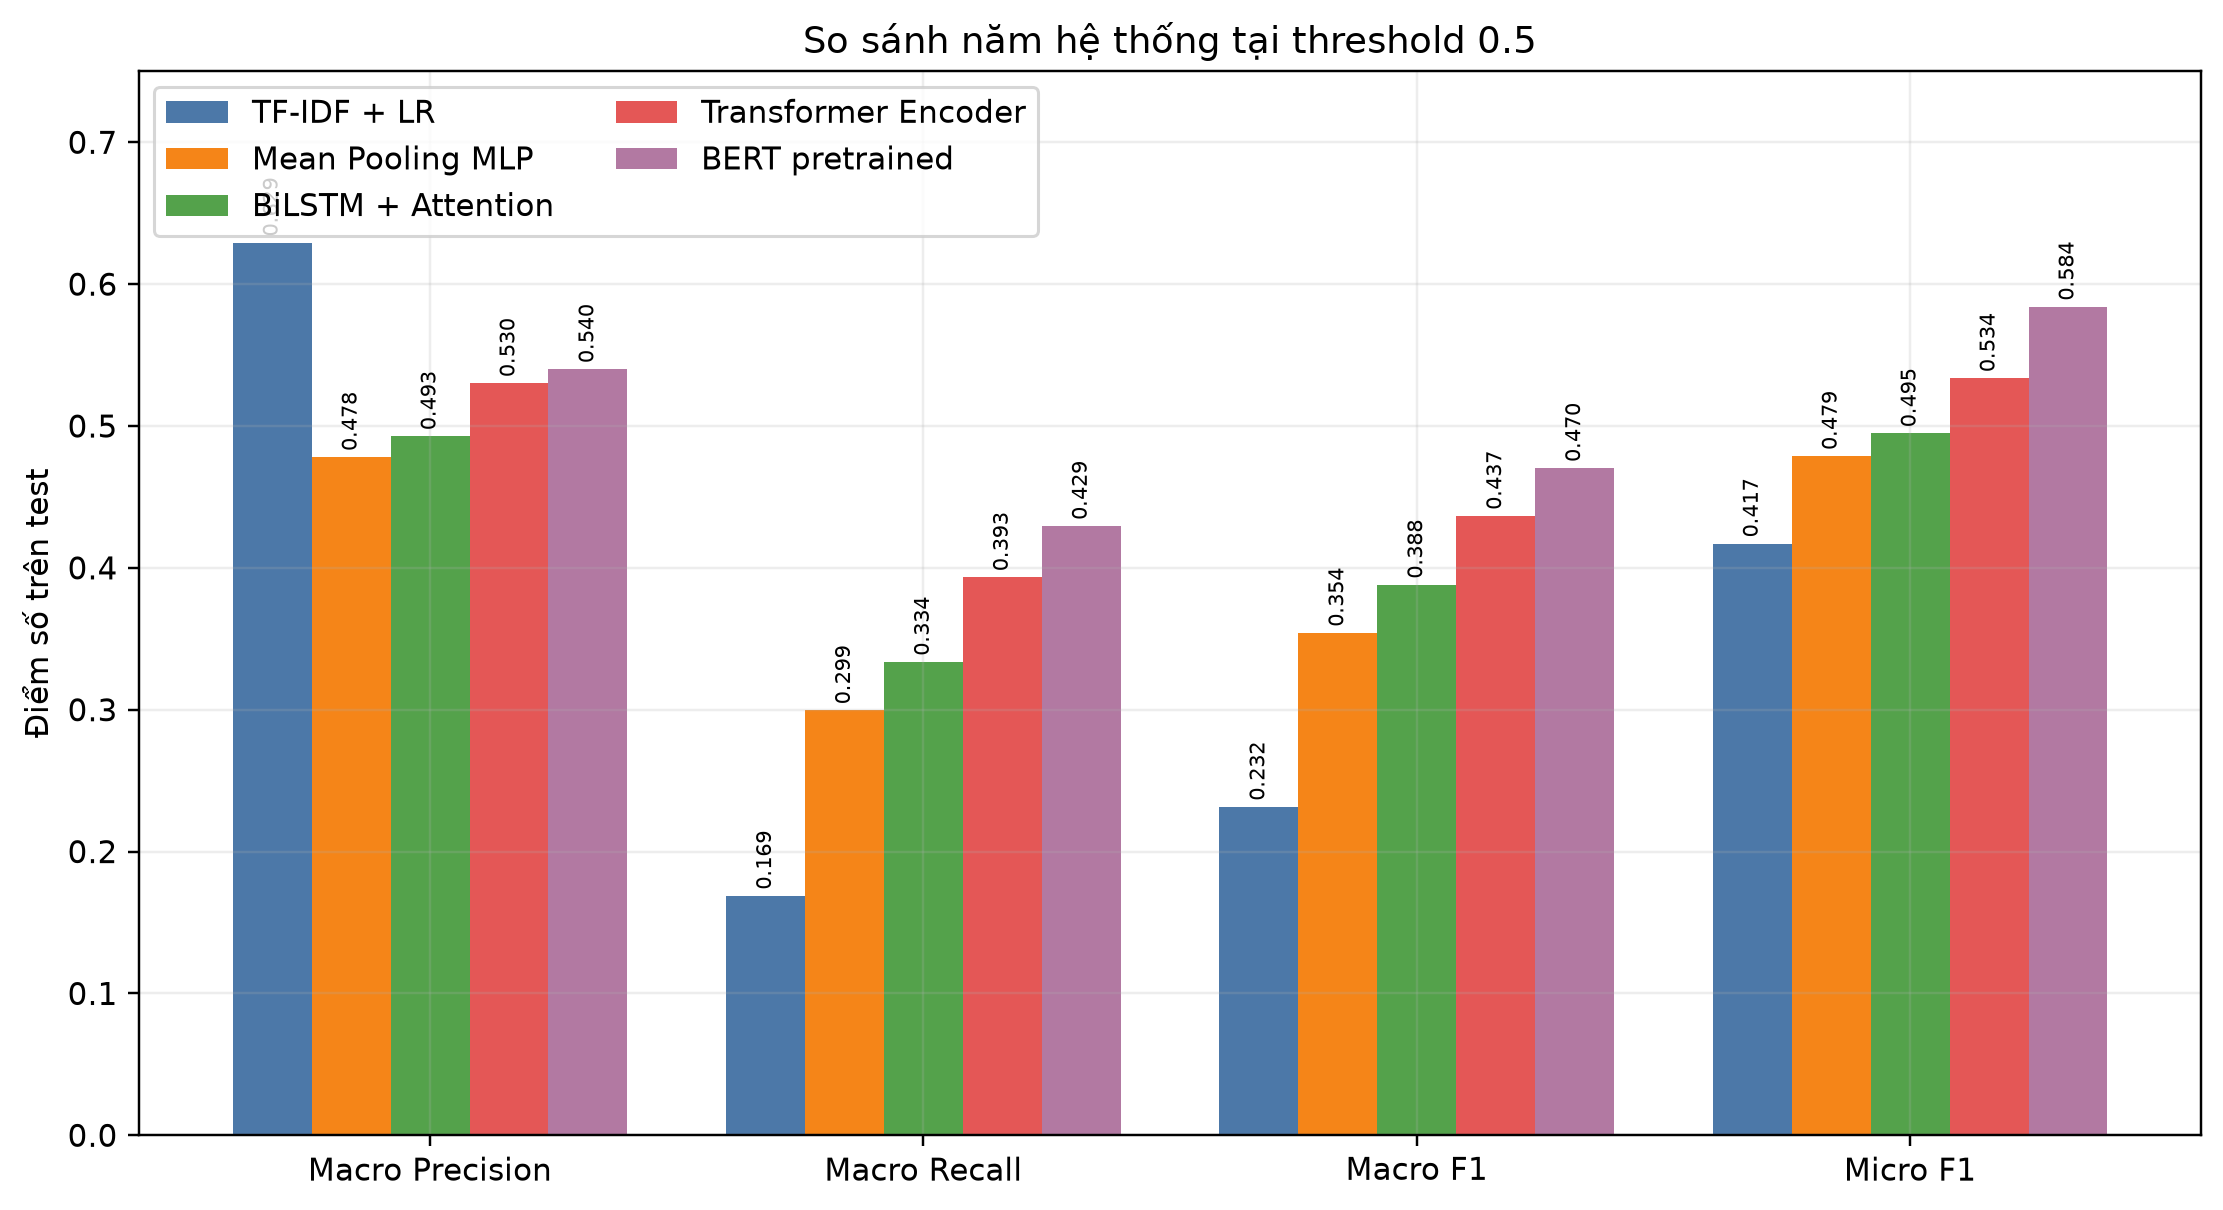
\includegraphics[width=0.98\textwidth]{model_comparison.png}
\caption{So sánh năm hệ thống tại threshold 0.5}
\label{fig:model-comparison}
\end{figure}

\subsection{Kết quả sau threshold tuning}

Bảng~\ref{tab:threshold-results} và Hình~\ref{fig:threshold-study} cho thấy threshold ảnh hưởng tới mọi kiến trúc. TF-IDF cải thiện lớn nhất, từ 0.2315 lên 0.4301 macro-F1, vì threshold 0.5 ban đầu làm recall quá thấp. Per-label thresholds hạ ranh giới cho nhiều nhãn và khôi phục positive cases.

Đây là một kết quả đáng chú ý: TF-IDF sau tuning vượt MLP 0.3983 và BiLSTM 0.4095. GoEmotions chứa nhiều lexical cues trực tiếp như từ ngữ biểu thị biết ơn, yêu thích, xin lỗi hoặc tức giận; một mô hình tuyến tính vẫn có thể khai thác tốt các tín hiệu này. Kết quả cho thấy baseline đơn giản nhưng có decision threshold phù hợp không nên bị đánh giá thấp, đồng thời bác bỏ cách diễn giải máy móc rằng kiến trúc càng phức tạp thì luôn càng tốt.

MLP tăng từ 0.3541 lên 0.3983; BiLSTM từ 0.3880 lên 0.4095; Transformer từ 0.4366 lên 0.4679; BERT từ 0.4703 lên 0.4976. Cả năm chọn per-label thresholds bằng validation macro-F1. Với BiLSTM, global threshold tình cờ đạt test 0.4097, cao hơn per-label 0.0002, nhưng không được đổi strategy theo test vì sẽ gây rò rỉ thông tin đánh giá.

\begin{figure}[H]
\centering
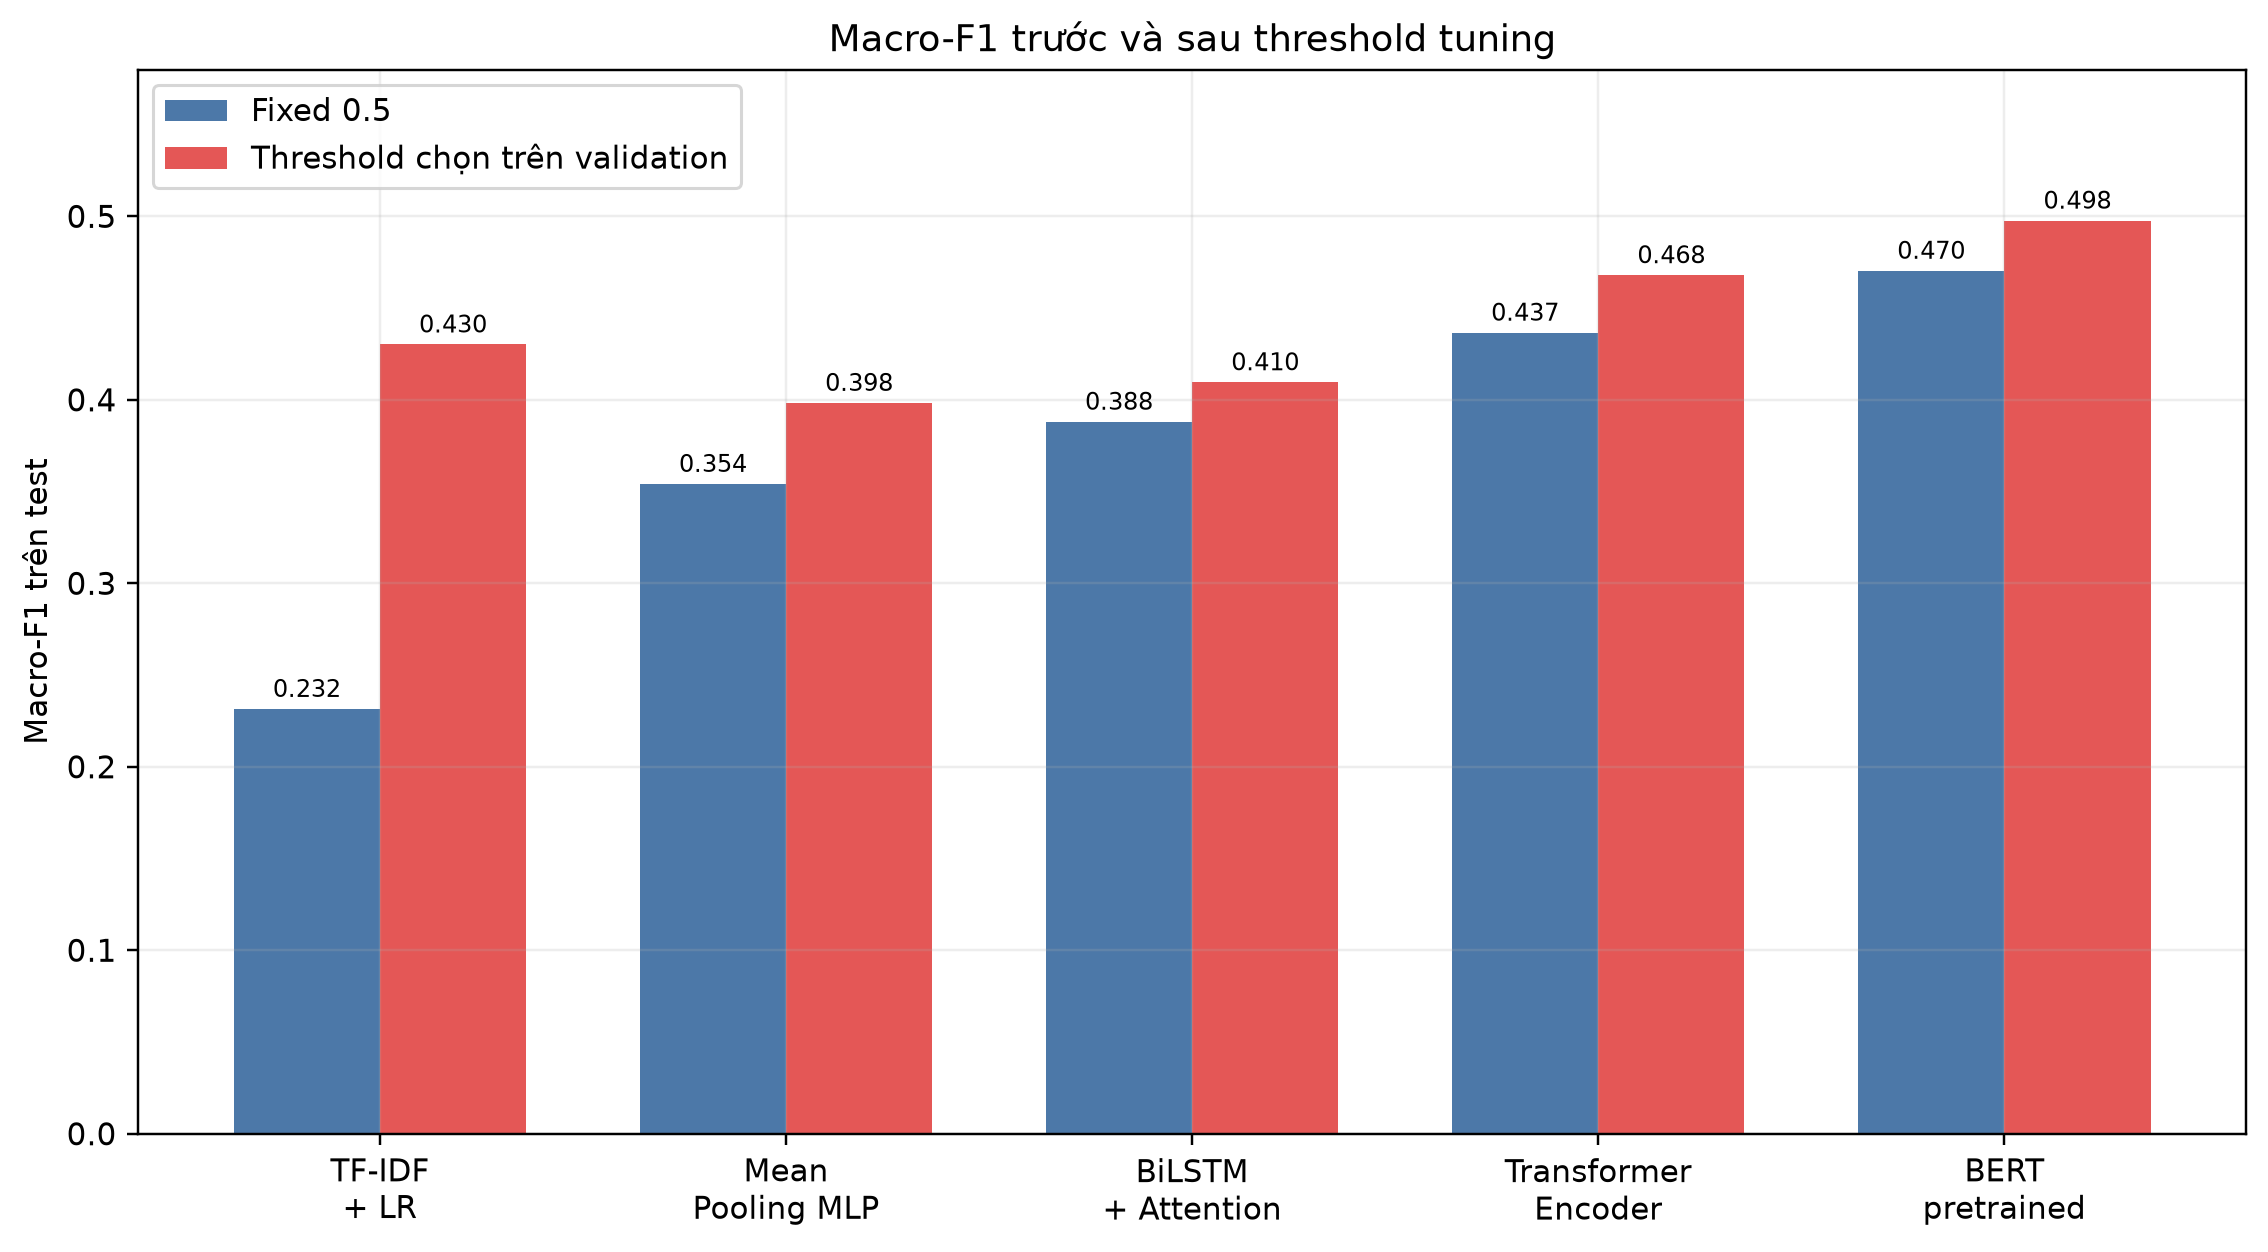
\includegraphics[width=0.98\textwidth]{threshold_study.png}
\caption{Macro-F1 tại fixed 0.5 và sau threshold tuning cho năm hệ thống}
\label{fig:threshold-study}
\end{figure}

Sau tuning, Transformer train-from-scratch đạt 0.4679, gần BERT fixed 0.5 là 0.4703. So sánh công bằng nhất vẫn là tuned với tuned: BERT 0.4976 cao hơn Transformer 0.0297. Calibration tốt thu hẹp một phần khoảng cách, nhưng pretrained language knowledge vẫn có lợi thế.

Micro-F1 không luôn tăng cùng macro-F1. BERT tuned có macro-F1 cao hơn nhưng micro-F1 0.5826 thấp hơn nhẹ fixed 0.5840. Đây là trade-off khi tiêu chí chọn ưu tiên đều 28 nhãn: model phát hiện thêm nhãn hiếm nhưng có thể tạo thêm false positives tổng thể.

\subsection{Ảnh hưởng của \texttt{pos\_weight}}

Project cũng thử xử lý mất cân bằng bằng cách huấn luyện Transformer với \texttt{BCEWithLogitsLoss(pos\_weight)}. Với nhãn $j$, trọng số positive được tính từ train theo $w_j^+=\min(N_j^-/N_j^+,50)$; do đó lỗi bỏ sót nhãn hiếm bị phạt mạnh hơn, còn giới hạn 50 tránh trọng số quá lớn. Đây là một biến thể loss của cùng Transformer, không phải một kiến trúc độc lập trong bảng so sánh năm hệ thống.

\begin{table}[H]
\centering
\small
\begin{tabular}{llrrr}
\toprule
\textbf{Loss} & \textbf{Threshold} & \textbf{Macro P} & \textbf{Macro R} & \textbf{Macro F1} \\
\midrule
BCE thường & Fixed 0.5 & 0.5301 & 0.3933 & 0.4366 \\
BCE thường & Per-label tuned & 0.5128 & 0.4725 & 0.4679 \\
BCE + \texttt{pos\_weight} & Fixed 0.5 & 0.2850 & 0.6287 & 0.3779 \\
BCE + \texttt{pos\_weight} & Per-label tuned & 0.3880 & 0.5207 & 0.4360 \\
\bottomrule
\end{tabular}
\caption{Ảnh hưởng của \texttt{pos\_weight} và threshold trên Transformer}
\label{tab:pos-weight-results}
\end{table}


Tại threshold 0.5, \texttt{pos\_weight} tăng macro recall từ 0.3933 lên 0.6287 nhưng làm macro precision giảm từ 0.5301 xuống 0.2850, nên macro-F1 giảm từ 0.4366 còn 0.3779. Sau per-label threshold tuning, phiên bản có trọng số đạt 0.4360, vẫn thấp hơn 0.4679 của BCE thường. Kết quả cho thấy tăng chi phí false negative giúp model nhạy hơn với positive labels nhưng đồng thời tạo quá nhiều false positives; trong cấu hình hiện tại, BCE thường kết hợp threshold tuning cân bằng precision và recall tốt hơn.

\subsection{Phân tích theo từng nhãn}

Hình~\ref{fig:per-label} minh họa Transformer trước và sau per-label tuning. Có 19/28 nhãn cải thiện, 6 giảm và 3 giữ nguyên. Các mức tăng đáng chú ý gồm \textit{grief}, \textit{caring}, \textit{annoyance}, \textit{disappointment} và \textit{anger}. Một threshold chung không phù hợp với nhãn có tần suất và phân bố probability khác nhau.

\begin{figure}[H]
\centering
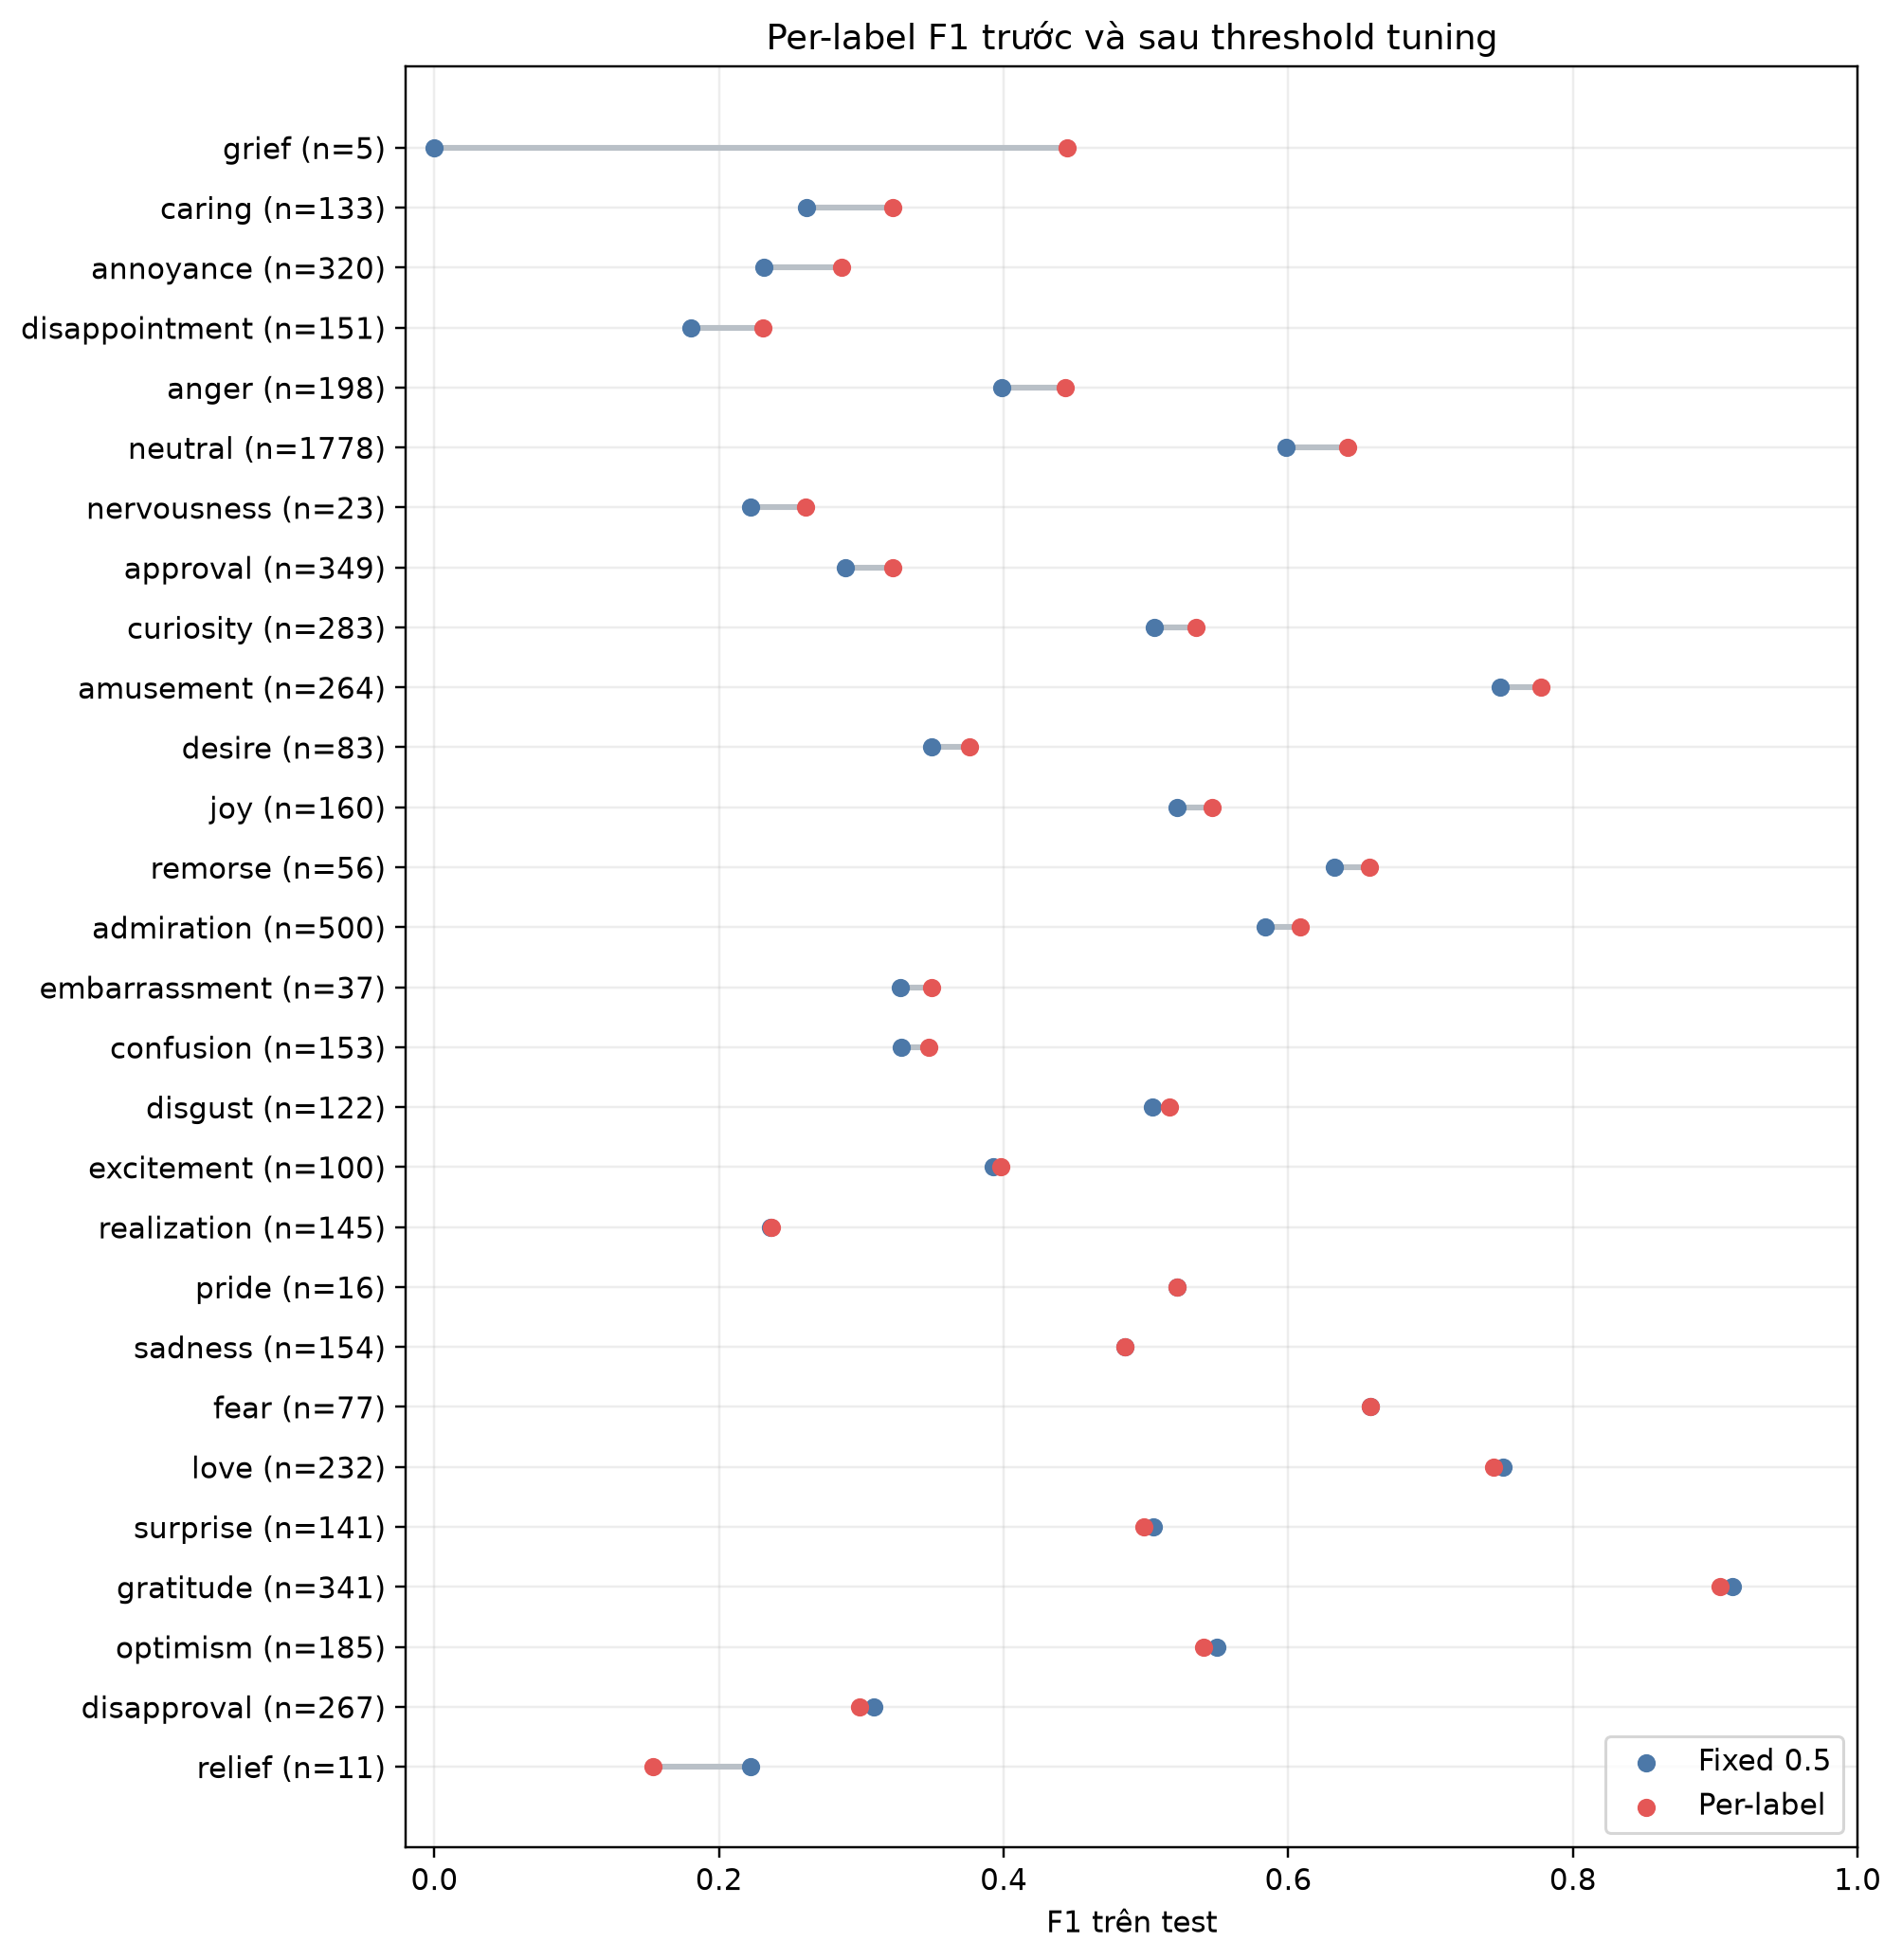
\includegraphics[width=0.86\textwidth]{per_label_f1.png}
\caption{Per-label F1 của Transformer trước và sau threshold tuning}
\label{fig:per-label}
\end{figure}

Thay đổi lớn ở nhãn cực hiếm cần đọc thận trọng. Test chỉ có 5 positive samples cho \textit{grief} và 11 cho \textit{relief}; vài dự đoán đã làm F1 biến động mạnh. Per-label tuning cải thiện điểm hiện tại nhưng chưa chứng minh threshold ổn định trên dữ liệu khác.

\subsection{Phân tích theo đặc điểm mẫu}

Hình~\ref{fig:slices} so sánh ba mô hình train-from-scratch theo độ dài câu và số nhãn thật. Sample-level F1 giảm khi câu dài hơn và label cardinality tăng. Trên sáu nhóm, Transformer cao hơn BiLSTM và MLP, phù hợp với khả năng self-attention trao đổi thông tin giữa nhiều vị trí.

\begin{figure}[H]
\centering
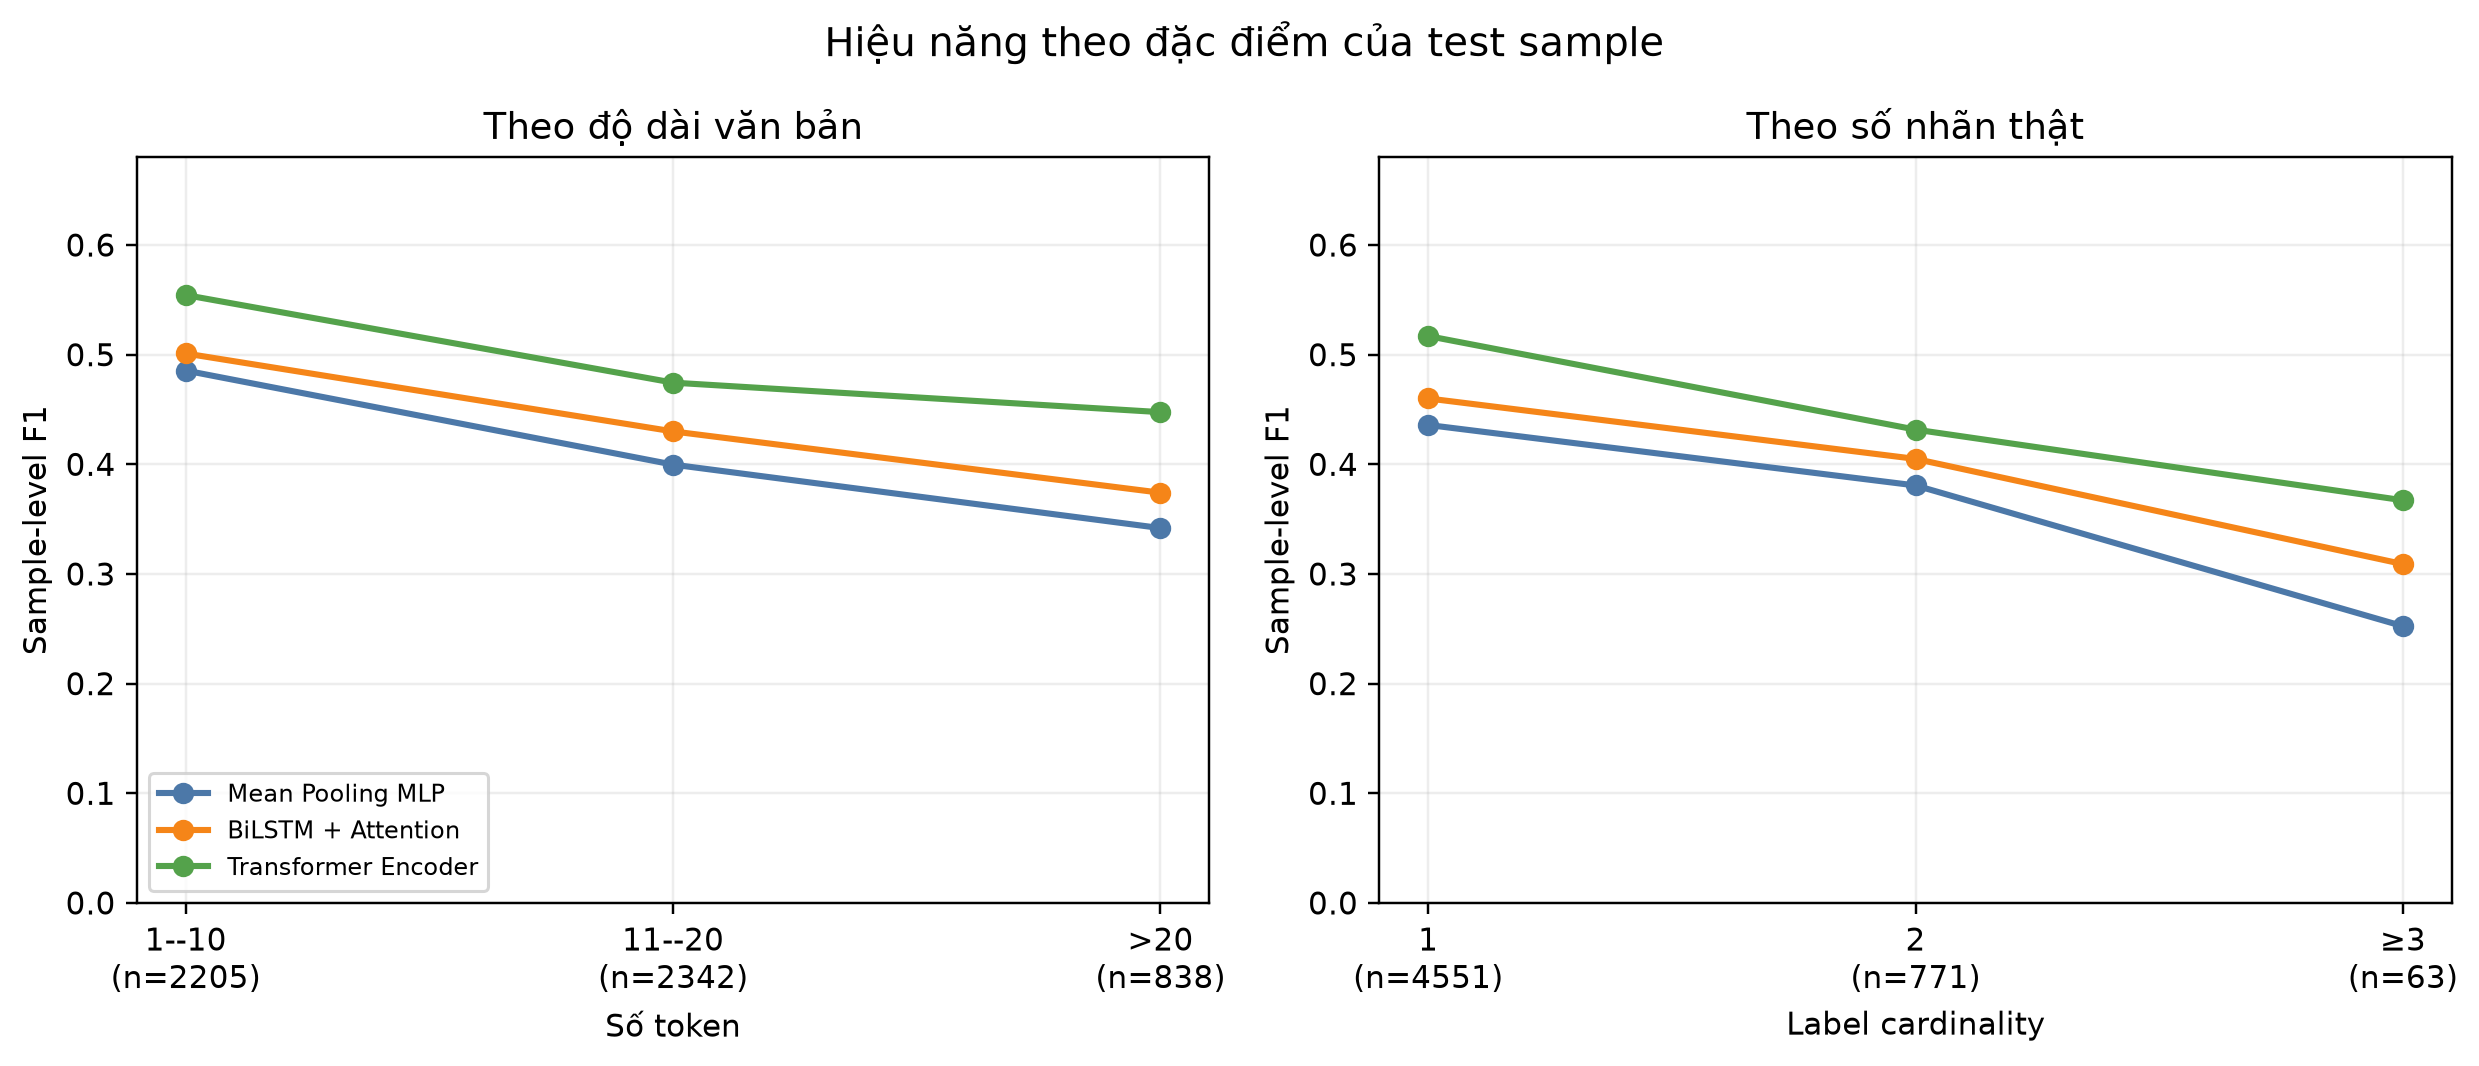
\includegraphics[width=0.99\textwidth]{slice_performance.png}
\caption{Sample-level F1 theo độ dài và label cardinality}
\label{fig:slices}
\end{figure}

Nhóm có từ ba nhãn trở lên chỉ gồm 63 test samples nên kết quả mang tính mô tả. Cả ba model giảm khi số nhãn tăng. Model thường nhận ra cảm xúc nổi bật nhất nhưng bỏ sót nhãn phụ hợp lý.

\subsection{Các failure modes chính}
\begin{table}[H]
\centering
\footnotesize
\begin{tabular}{p{5.2cm}p{3.0cm}p{3.0cm}p{2.2cm}}
\toprule
\textbf{Văn bản} & \textbf{Nhãn thật} & \textbf{Dự đoán} & \textbf{Nhóm lỗi} \\
\midrule
Not sure why [NAME] didn't foul to stop the fast break there & neutral & confusion, neutral & Negation \\
I was teased for being a virgin when I was a 6th grader- in 2005 & embarrassment & realization & Bỏ sót nhãn hiếm \\
Hi, [NAME]! I thought I would stop by and wish you a wonderful and prosperous year! Have a good one! -HappyFriendlyBot & caring, love, optimism & caring & Nhiều nhãn \\
I’m really sorry about your situation :( Although I love the names Sapphira, Cirilla, and Scarlett! & sadness & love, remorse & Mơ hồ/nhãn gần nghĩa \\
\bottomrule
\end{tabular}
\caption{Một số lỗi của Transformer với per-label thresholds}
\label{tab:error-examples}
\end{table}


Bảng~\ref{tab:error-examples} minh họa phủ định, bỏ sót nhãn hiếm, mẫu nhiều nhãn và cảm xúc gần nghĩa. Với phủ định, model có thể chú ý từ khóa cảm xúc nhưng chưa biểu diễn đúng phạm vi của \textit{not} hoặc \textit{never}. Với mẫu nhiều nhãn, model thường chỉ chọn tín hiệu rõ nhất.

Các cặp \textit{sadness}/\textit{remorse}, \textit{excitement}/\textit{optimism} và \textit{gratitude}/\textit{admiration} có ranh giới gần. Ví dụ dùng để giải thích hành vi, không thay thế thống kê toàn test và không chứng minh nguyên nhân nội tại của model.

\section{Hạn chế}

\begin{itemize}

\item Việc so sánh BERT pretrained với các mô hình train-from-scratch chưa hoàn toàn cân bằng, do BERT đã được tiền huấn luyện trên lượng dữ liệu lớn và có quy mô mô hình lớn hơn đáng kể.

\item Quá trình gán nhãn cảm xúc mang tính chủ quan nhất định. Một số nhãn có nội dung gần nhau hoặc chồng lấn, trong khi các câu Reddit thường ngắn và có thể thiếu ngữ cảnh cần thiết để xác định cảm xúc một cách rõ ràng.

\item Đối với các nhãn rất hiếm, số lượng mẫu trong tập test còn hạn chế, khiến các chỉ số đánh giá có thể biến động mạnh và kém ổn định.

\item Chiến lược per-label threshold sử dụng 28 ngưỡng độc lập, tương ứng với 28 bậc tự do, nên có nguy cơ khớp quá mức với tập validation. Cách tiếp cận này thực chất tối ưu decision rule theo F1-score, chứ không phải hiệu chỉnh xác suất (probability calibration) theo nghĩa chặt như temperature scaling hoặc isotonic regression.

\end{itemize}


\section{Kết luận}

Project đã xây dựng một pipeline hoàn chỉnh cho bài toán emotion classification, bao gồm kiểm tra dữ liệu, tạo các tập dữ liệu sạch, tokenization, xây dựng vocabulary, mã hóa nhãn multi-hot, huấn luyện và đánh giá năm hệ thống khác nhau. Quy trình thực nghiệm được kiểm soát thống nhất bằng cách chỉ fit vocabulary và representation trên tập train, lựa chọn checkpoint và threshold dựa trên tập validation, đồng thời giữ tập test hoàn toàn độc lập cho bước đánh giá cuối cùng. Cách thiết lập này giúp bảo đảm tính nhất quán và hạn chế rò rỉ thông tin giữa các giai đoạn.

Trong ba mô hình nơ-ron được huấn luyện từ đầu, Transformer đạt kết quả tốt nhất với tuned macro-F1 0.4679, cao hơn MLP ở mức 0.3983 và BiLSTM ở mức 0.4095. Tuy nhiên, TF-IDF kết hợp Logistic Regression cải thiện đáng kể từ macro-F1 0.2315 tại threshold 0.5 lên 0.4301 sau khi tối ưu per-label thresholds, qua đó vượt cả MLP và BiLSTM. Kết quả này cho thấy các lexical cues vẫn đóng vai trò quan trọng trong bài toán emotion classification, đồng thời nhấn mạnh rằng một baseline tuyến tính đơn giản nhưng được lựa chọn decision rule phù hợp vẫn có thể đạt hiệu quả cạnh tranh.

BERT pretrained đạt kết quả tốt nhất trong toàn bộ các hệ thống, với macro-F1 0.4703 khi sử dụng threshold 0.5 và tăng lên 0.4976 sau threshold tuning. Nhìn chung, kết quả cho thấy cả chất lượng representation lẫn decision rule đều có ảnh hưởng đáng kể đến hiệu năng cuối cùng. Threshold tuning có thể làm thay đổi rõ rệt thứ hạng giữa các mô hình; Transformer cung cấp biểu diễn tốt nhất trong nhóm neural model tự xây dựng, trong khi pretraining giúp BERT duy trì lợi thế khi các hệ thống được so sánh dưới cùng một quy trình tuning.

Các lỗi còn lại chủ yếu xuất hiện ở những nhãn có ít mẫu, các cảm xúc có ý nghĩa gần nhau, câu dài và các trường hợp chứa đồng thời nhiều nhãn cảm xúc. Trong tương lai, có thể mở rộng thực nghiệm bằng cách đánh giá mô hình trên nhiều random seed để kiểm tra độ ổn định của kết quả, phân tích mức độ ổn định của per-label thresholds giữa các lần huấn luyện, đồng thời khai thác mối quan hệ giữa các nhãn thay vì xem 28 nhãn cảm xúc như những quyết định hoàn toàn độc lập.


\begin{thebibliography}{9}
\bibitem{demszky2020} D. Demszky et al., ``GoEmotions: A Dataset of Fine-Grained Emotions,'' \textit{Proceedings of ACL}, pp. 4040--4054, 2020. DOI: \href{https://doi.org/10.18653/v1/2020.acl-main.372}{10.18653/v1/2020.acl-main.372}.
\bibitem{hochreiter1997} S. Hochreiter and J. Schmidhuber, ``Long Short-Term Memory,'' \textit{Neural Computation}, vol. 9, no. 8, 1997.
\bibitem{bahdanau2015} D. Bahdanau, K. Cho, and Y. Bengio, ``Neural Machine Translation by Jointly Learning to Align and Translate,'' \textit{ICLR}, 2015.
\bibitem{vaswani2017} A. Vaswani et al., ``Attention Is All You Need,'' \textit{NeurIPS}, vol. 30, 2017.
\bibitem{devlin2019} J. Devlin, M.-W. Chang, K. Lee, and K. Toutanova, ``BERT: Pre-training of Deep Bidirectional Transformers for Language Understanding,'' \textit{NAACL-HLT}, pp. 4171--4186, 2019.
\end{thebibliography}
\end{document}
